\chapter{Results}

This chapter reports on the evaluation and application of statistical methods presented in the Methods (Section \ref{Novel Statistical}). I first evaluated the statistics on simulated data. Having selected statistical measures based on validation with data consistent with the null hypothesis, I applied my methods to naturally occurring cases of the alternate hypothesis, aiming to validate whether they do, in fact, reflect an elevated level of disequilibrium. I report the application of my methods to two biological cases with striking prior evidence for recent perturbations affecting: an entire genome (loss of DNA methylation in \textit{D. melanogaster}); or, a small genomic segment (\textit{Fxy} in \textit{M. musculus}). I find that the methods are consistent with prior predictions made with knowledge of mechanism alone. Applying the methods to the evolution of humans, I discover that the majority of the human genome is not at mutation equilibrium.

\section{Developing and validating the methods}
\label{Simulation}

The process of validation began using the synthetic data sets in which the generating process is known to be in equilibrium. For some statistics, it was necessary to establish their properties on alignments that range in their evolutionary divergence, for this I used the observed Microbial data set.  

\subsubsection{The best method of model fitting is without initialisation}

A necessary precursor to the application of any methods was to establish approximately optimal fits of the models. Initialisation is the process of using the parameter estimates from a nested model fit  as initial estimates. The initialisation experiment revealed that there are no intrinsic problems with the fitting process for GN or GNS. A fit was considered poor if the log-likelihood from the initialised method was higher than that of the uninitialised method. There were no occurrences of poor fits for any of the synthetic alignments. Initialised fits which were faster than the corresponding uninitialised fits were rare, occurring at a rate of about ~1\%. Based on these results, all subsequent model fitting is without initialisation.

\subsection{The Test of Existence (TOE) with parametric bootstrapping provided a robust estimation of significance}
\label{TOE_results}

The TOE is a LRT for the existence of disequilibrium on a single edge, a further description is provided in the Methods (Section \ref{Test of Existence}).  
To determine whether a given LRT statistic is significant requires establishing the appropriate null distribution. Statistical theory states that under certain conditions, the LRT statistic will be $\chi^2_{df}$ distributed with degrees freedom (df) equal to the difference in the number of free parameters between the models. In which case, one can obtain the $p$-values for a given LRT statistic simply from the analytical distribution. The behaviour of the TOE with real finite data is unknown. 

There were no conditions under which the $\hat p$-values were consistent with the theoretical expectations (Figure \ref{fig:synthetic/lrt/197113-long_seq}). The figure shows data generated from the same High JSD, High Entropy seed, however, the results for all seeds were very similar (Figure \ref{fig:synthetic/lrt/all-seeds}). For alignments of length 300bp (Figure \ref{fig:synthetic/lrt/197113-long_seq}a), the distribution of TOE statistic yields an excess of small $\hat p$-values, evident at data points of the Quantile-Quantile plot being well below the expected diagonal. Increasing statistical power by using longer alignments (Figure \ref{fig:synthetic/lrt/197113-long_seq}b), ameliorated this but did not resolve it.  

\begin{figure}[htbp]
\centering
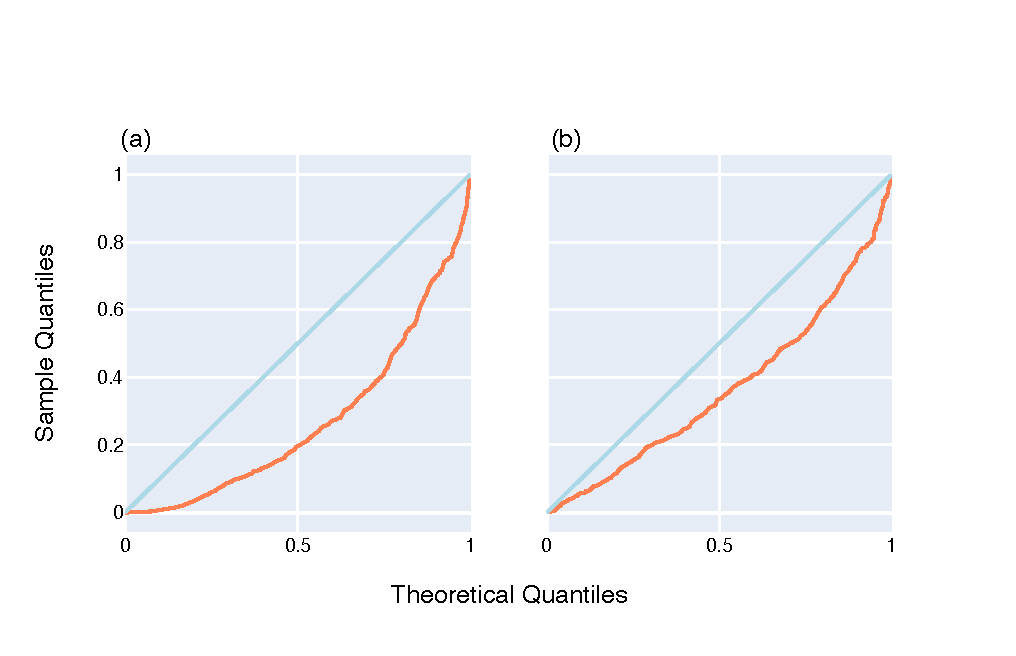
\includegraphics[width=\textwidth]{figures/plots/synthetic/lrt/197113_332182_17210-long_seq.pdf}
\caption[Increasing the length of the alignments gives a distribution of $\hat p-$ values closer, but not consistent with theoretical expectations]{\textbf{Increasing the length of the alignments gives a distribution of $\hat p-$ values closer, but not consistent with theoretical expectations.} The Quantile-Quantile (Q-Q) plots compare the $\hat p$-value distribution of the test for existence in stationary simulated data to the uniform distribution (pink line). Theoretical expectation is illustrated by the diagonal (blue line). Q-Q plot for \textbf{(a)} synthetic alignments of length $300$bp, \textbf{(b)}, synthetic alignments of length $30,000$bp. Each data set contains 1,000 synthetic stationary alignments. Both data sets shown are generated from the same high JSD, high entropy seed. The other seeds exhibited the same pattern, the result is shown in the appendix Figure \ref{fig:synthetic/lrt/all-seeds}.}
\label{fig:synthetic/lrt/197113-long_seq}
\end{figure}

The results in Figure \ref{fig:synthetic/lrt/197113-long_seq} demonstrate that I cannot assume the TOE statistic to be $\chi^{2}$ distributed. As conventional asymptotic approximations to the TOE distribution were shown not to hold, $\hat p$-values were estimated via parametric bootstrap. 

\subsection{A transformed $\nabla$ statistic exhibited robust behaviour under the null}
\label{nabla_results}

$\nabla$ is a measure of the speed of convergence of the substitution process to equilibrium, a detailed description of $\nabla$ is provided in the Methods (Section \ref{nabla}). 

The $\nabla$ statistic from a stationary process was sensitive to alignment length. Presented in Figure \ref{fig:synthetic/d-conv-vs-conv/HighJSDHighEntropy}a are the distributions of $\hat \nabla$ in simulated data sets generated by the same stationary seed, but for alignments of length 300bp, 3,000bp, and 30,000bp. Figure \ref{fig:synthetic/d-conv-vs-conv/HighJSDHighEntropy}a shows that not only was there more variation in $\hat \nabla$ for the shorter alignments, but the location of the mean was inversely proportional to alignment length. This effect held for all seeds (Figure \ref{fig:synthetic/conv/all_seeds}). Since empirical applications must compare statistics between sequences of different lengths, the $\nabla$ statistic required a transformation. 

\begin{figure}[htbp]
\centering
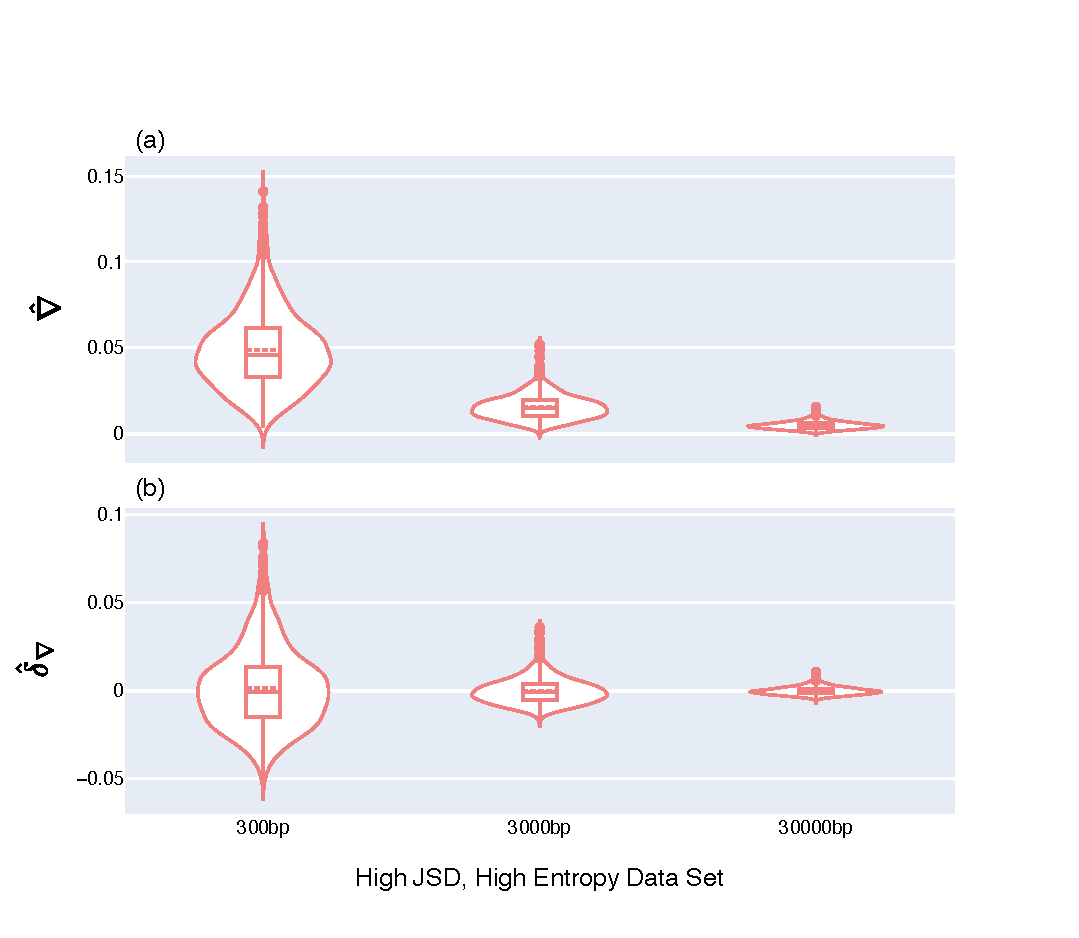
\includegraphics[width=\textwidth]{figures/plots/synthetic/d-conv-vs-conv/High JSD, High Entropy.pdf}
\caption{\textbf{The transformed statistic, $\delta_\nabla$, corrects for error introduced by the length of the alignment.} The violin plots show the distribution of $\hat \delta_\nabla$ for simulated data sets of alignment length 300, 3,000, and 30,000. \textbf{(a)} The original statistic, $\nabla$, had both a higher level of variation and a higher expected value in shorter sequences. \textbf{(b)} The transformed statistic $\delta_\nabla$ corrects for the location of the expected value only. The variation in shorter sequences remains, however, the mean for alignments of all lengths is centred on zero. Each data set contains 1,000 synthetic stationary alignments. The High JSD, High Entropy seed is shown, however, this result was the same for all seeds, included in the appendix (see Figure \ref{fig:synthetic/conv/all_seeds}). }
\label{fig:synthetic/d-conv-vs-conv/HighJSDHighEntropy}
\end{figure}

The selected transformation denoted $\delta_\nabla$, adjusted for location only, ensuring the expected value was zero when the null was true. For a given alignment, $\hat \delta_\nabla$ is the difference between the observed $\hat \nabla$ and the mean of $\hat \nabla$ from synthetic alignments generated under the null, $\hat \delta_\nabla =  \hat\nabla - \mu_{\hat \nabla{null}}.$ The distributions of $\hat \delta_\nabla$ in simulated data shows that the expected value of the transformed $\delta_\nabla$ statistic is close to zero when the null is true (Figure \ref{fig:synthetic/d-conv-vs-conv/HighJSDHighEntropy}b). Although there is more variation in the shorter sequences, this simple method of transformation was chosen because the statistic retains the same units as the untransformed statistic. 

When applied to the observed Microbial, $\delta_\nabla$ increases with a known marker of historic disequilibrium. As described in the methods, JSD is an information-theoretic measure of the difference between probability distributions. Throughout, I have relied on compositional attributes as an implication for the existence of disequilibrium, with the caveat that it may have been strictly historic. Unlike the simulated data, for the observed Microbial data set shown in this scatter plot, I expect varied disequilibrium in a proportion of the taxa. The $\delta_\nabla$ statistic has a strong positive relationship with the JSD between ingroup edges, illustrated in Figure \ref{fig:microbial/d-conv/JSD}. This relationship is very encouraging as it supports that $\delta_\nabla$ is in fact measuring what it is intended to measure, mutation disequilibrium. 

\begin{figure}[htbp]
\centering
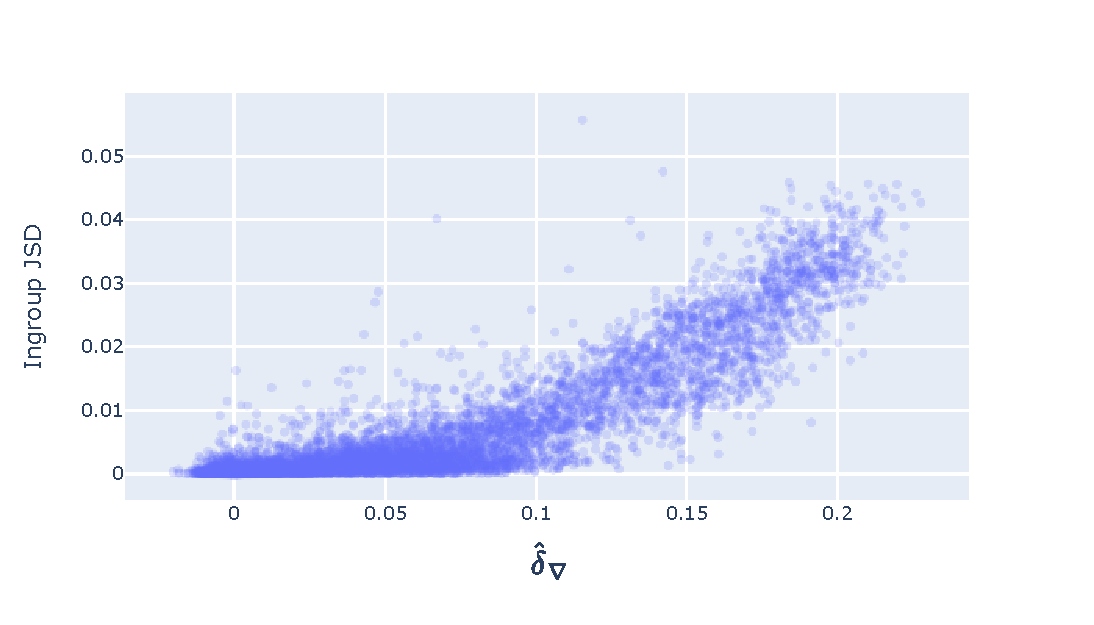
\includegraphics[width=\textwidth]{figures/plots/microbial/d-conv-JSD.pdf}
\caption{\textbf{The $\hat\delta_\nabla$ statistic increased with a marker of historic disequilibrium.} The scatter plots shows magnitude of disequilibrium measure by $\hat\delta_\nabla$ and the JSD between ingroup taxa for the observed Microbial data set. The Microbial data set comprises 9702 alignments where the level of disequilibrium is expected to vary.}
\label{fig:microbial/d-conv/JSD}
\end{figure}

\subsection{The $T_{50}$ statistic exhibited paradoxical properties that prevented interpretation}
\label{T50_results}

$T_{50}$ is a measure of the distance to halfway to equilibrium, measured in terms of the expected number of substitutions, a detailed description of $T_{50}$ is provided in the Methods (Section \ref{T50}). 

The algorithmic routines used in calculating the $T_{50}$ statistic were vulnerable to machine precision errors. The testing of $T_{50}$ illustrated a simple error that can arise from calculations using \gls{floating-point arithmetic}. Consider the following equation, $1e16 + 1.0 - 1e16$. This should equal $1$, however, using a computer it will evaluate to $0$. Such is a simple example of how the representation of numbers in computers can propagate errors in calculations. One test case for $T_{50}$ was, given model parameters generated by GTR where the nucleotide distribution is stationary, the returned value should be $0$. Interestingly, this test was failing. Debugging revealed that the failure was due to machine precision errors. Following this discovery, code for $T_{50}$ was changed to use accurate algorithms for floating-point sums and dot products \citep{accupy}. These algorithms avoid possible imprecision by tracking multiple intermediate partial sums, a routine that does come with a modest speed loss \citep{Shewchuk1997AdaptivePredicates, Ogita2005AccurateProduct}. 

Even using the most precise algorithms, the estimation of $T_{50}$ was extremely vulnerable to sampling error. The simulated data was generated to be stationary and the expected $T_{50} = 0$. The error was unmistakable in data generated by the High JSD, Low Entropy seed, shown in Figure \ref{fig:T50-short_long}, where the outlying values for shorter alignments completely obscure the shape of the distributions. Although most pronounced in the seed shown, higher sampling error in the shorter sequences was a feature of all seeds, (see Figure \ref{fig:synthetic/T50/all-seeds}). 

\begin{figure}[!ht]
\centering
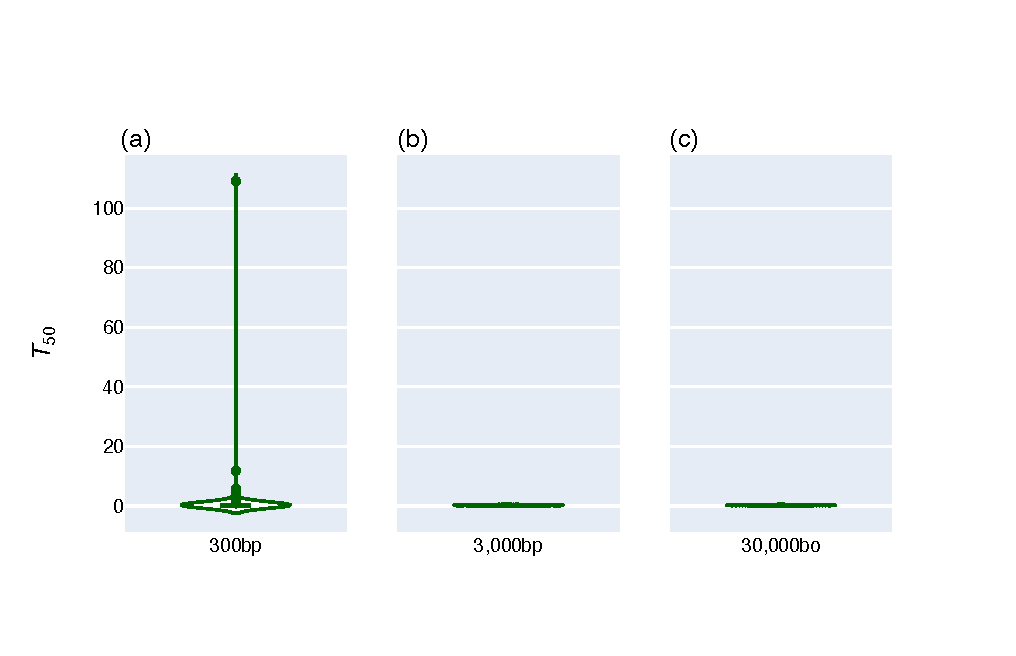
\includegraphics[width=\textwidth]{figures/plots/synthetic/T50/HighJSDLowEntropy-seq_len.pdf}\caption{\textbf{Long Alignments have less sampling error}}
\label{fig:T50-short_long}
\end{figure}

$T_{50}$ estimated under the null was not robust to features of the data. In the simulated stationary data, $T_{50}$ was sensitive to all conditions considered, JSD, entropy and length. It was highest in the low JSD seeds. In five of six cases, when grouped by length and entropy, the median $\hat T_{50}$ for low JSD was greater than the median $\hat T_{50}$ for high JSD (Figure \ref{t50_means}). Recall that JSD is used throughout as a marker of historic disequilibrium. Even though in the simulated data the foreground edge is stationary, it was expected that in the high JSD data sets there would be more disequilibrium in the background edges. It is thus unexpected both that there is a pattern, and that the pattern reflects higher disequilibrium in the low JSD data. $T_{50}$ was not considered further. 

\begin{table}[htbp]
\begin{tabularx}{\textwidth}{ 
  | >{\centering\arraybackslash}X
  | >{\centering\arraybackslash}X 
  | >{\centering\arraybackslash}X 
  | >{\centering\arraybackslash}X  
  | >{\centering\arraybackslash}X | }
\hline  
\textbf{Alignment Length} &\textbf{ High JSD, Low Entropy} & \textbf{ Low JSD, Low Entropy} & \textbf{High JSD, High Entropy} & \textbf{Low JSD, High Entropy} \\
\hline 
    \textbf{300bp} & 0.3184 & 0.3363 & 0.3497 & 0.4576 \\
    \textbf{3,000bp} & 0.2663 & 0.2563 & 0.3096 & 0.3990 \\
   \textbf{30,000bp} & 0.2514 & 0.2778 & .3107 & 0.3911 \\ 
\hline 
\end{tabularx}
\caption{\textbf{Median $\hat T_{50}$ for simulated stationary data sets.} In all but one case, when grouped by length and entropy, the median $\hat T_{50}$ for low JSD exceeded the median $\hat T_{50}$ for high JSD. Each data set contained 1,000 synthetic stationary alignments.}
\label{t50_means}

\end{table}


\subsection{Both tests of equivalence of process were consistent with asymptotic approximations}

As described in the Methods (Section \ref{Tests of Equivalence of Process}), the EOP tests are LR tests for whether related processes are shown to be different. This can be applied to two comparisons, adjacent and temporal. Adjacent is the test of equivalence between neighbouring alignments of the same edge, and temporal is the test between one-to-one orthologs. Both tests are a comparison of likelihoods between fitting both alignments with one $\mathrm{Q}$ (null), or fitting a separate $\mathrm{Q}$ per alignment (alternate). Significance is assessed with an LR, where again, it is necessary to determine whether asymptotic approximations apply. 

Applying both tests to their respective null distributions indicated that both were consistent with theoretical expectations (Figure \ref{fig:synthetic/adj-temp_eop/HighJSDHighEntropy}). Quantile-Quantile plots comparing the distribution of $\hat p$-values to the uniform distribution for the temporal test (Figure \ref{fig:synthetic/adj-temp_eop/HighJSDHighEntropy}a) and the adjacent test (Figure \ref{fig:synthetic/adj-temp_eop/HighJSDHighEntropy}b) established that the distribution of $\hat p-$values is almost indistinguishable from the uniform distribution. Based on this result I assume the statistic is $\chi^2_{df}$ distributed and in turn, obtained the $\hat p-$value from analytical distribution. 

\begin{figure}[htbp]
\centering
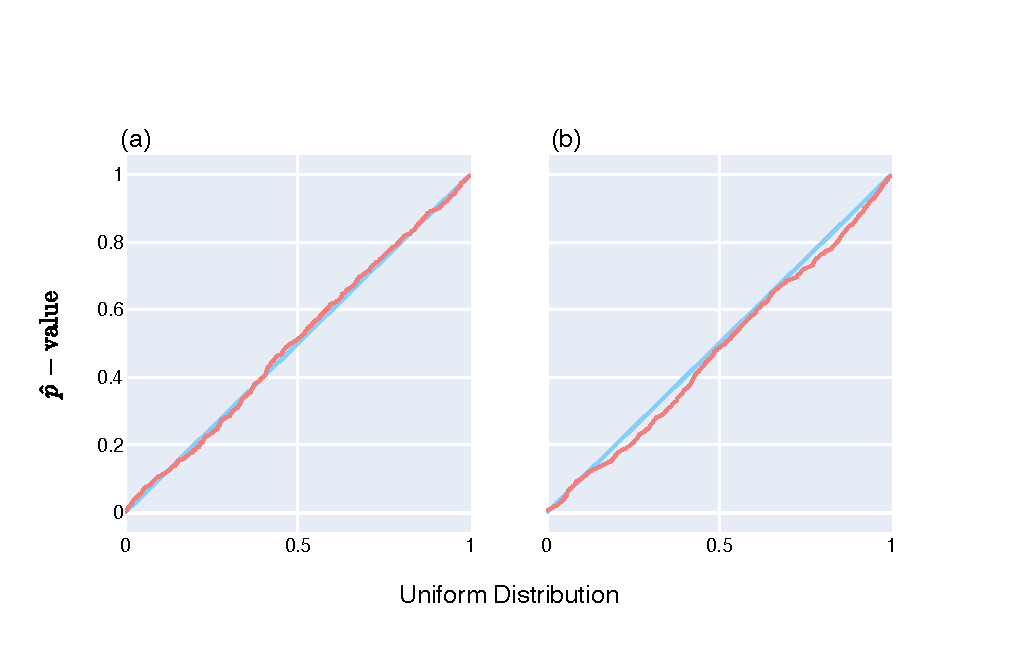
\includegraphics[width=\textwidth]{figures/plots/synthetic/adj-temp_eop/High JSD, High Entropy.pdf}
\caption{\textbf{Both equivalence of process tests were consistent with theoretical approximations.} The Quantile-Quantile plots compare the distribution of $\hat p-$values to the uniform distribution. As the data points (shown as the orange line) fall very close to the diagonal, this demonstrates that the distribution of $\hat p-$values is almost indistinguishable from the uniform distribution. (a) $\hat p-$values from temporal equivalence of process, (b) $\hat p-$values from adjacent equivalence of process. This result is shown for alignments of length 300 generated by the High JSD, High Entropy seed, however, the result was the same for all seeds and all lengths, shown in the appendix, see figure \ref{fig:synthetic/adj_eop/all_seeds} and \ref{fig:synthetic/temp_eop/all_seeds}.}
\label{fig:synthetic/adj-temp_eop/HighJSDHighEntropy}
\end{figure}

\section{Testing the known}

Having lost major components of the DNA methylation process that remain in its sister taxa, the \textit{D. melanogaster} genome is a natural occurrence of changed mutagenesis affecting the entire genome. $^5$mC is a well known hypermutable base. Consequently, the lack of $^5$mC in
\textit{D. melanogaster} led to the strong prediction that the \textit{D. melanogaster} genome would exhibit globally high levels of mutation disequilibrium. \textit{D. simulans} still methylates its DNA, which provided a necessary point of comparison. I performed two separate analyses with either \textit{D. melanogaster} or \textit{D. simulans} as the foreground. The analyses were applied to alignments of third codon positions from orthologous CDS. The expectations were that the \textit{D. melanogaster} genome would exhibit higher levels of both existence and magnitude of mutation disequilibrium than \textit{D. simulans} and that this would be a genome-wide relationship. The relative levels of purifying natural selection operating on the chromosomes allowed for further predictions regarding the magnitude of mutation disequilibrium. Specifically, that the X chromosome linked genes would exhibit a higher magnitude of mutation disequilibrium relative to autosomal genes. 

\subsection{The entire \textit{D. melanogaster} genome is systematically elevated in both the existence and magnitude of mutation disequilibrium compared to its sister taxa, \textit{D. simulans}}
\label{TOE_drosophila}

There is a striking elevation of the existence of mutation disequilibrium in the \textit{D. melanogaster} genome when compared to that of \textit{D. simulans} (Figure \ref{fig:drosophila_lrt_qq}). Each subplot in Figure \ref{fig:drosophila_lrt_qq} shows the distribution of TOE $\hat p$-values estimated from the observed data, as well as simulated positive and negative controls. The controls are two synthetic cases of ground truth: no disequilibrium (negative); and disequilibrium (positive). For an observed alignment, each data point from the positive and negative controls was simulated using parameter estimates of GN and GNS models respectively. The observed data points of \textit{D. melanogaster}, shown in Figure \ref{fig:drosophila_lrt_qq}b, fall substantially further from the -ve control than that of \textit{D. simulans}, shown in Figure \ref{fig:drosophila_lrt_qq}a. This indicates that, as specified by the TOE, a much larger proportion of the \textit{D. melanogaster} genome is in mutation disequilibrium than \textit{D. simulans}. 

\begin{figure}[h]
\centering
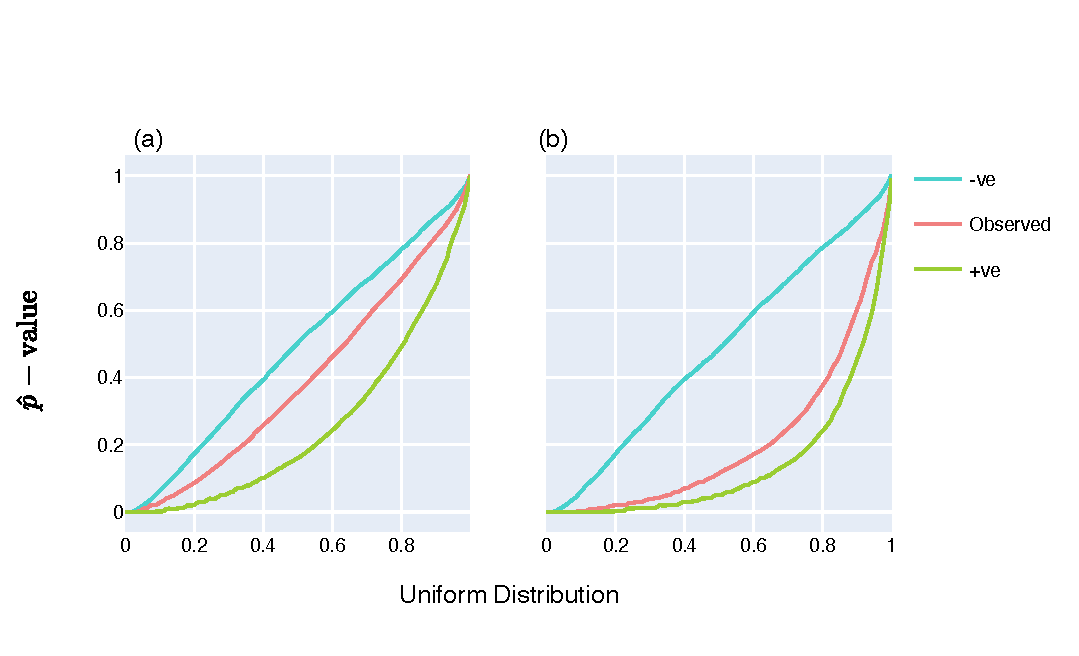
\includegraphics[width=	\textwidth]{figures/plots/drosophila/LRT-QQ.pdf}
\caption{}
\label{fig:drosophila_lrt_qq}
\end{figure}


Determining the specific proportion of disequilibrium for each genome requires correcting for multiple tests of the same hypothesis, however, the resolution of $\hat p$-values is too low for conventional methods of multiple test corrections. TOE $\hat p$-values were estimated using bootstraps for which compute time precludes greater precision. I calculated that to get sufficient replicates to apply a Bonferroni correction would take approximately $9,009$ hours per alignment. This is a level of computation that is both impractical and unnecessary. 

I established an alternate strategy that takes advantage of the shape of the distribution. The challenge of correcting for multiple tests is pronounced in genomics, for which \cite{Storey2003StatisticalStudies} introduced a formal procedure for estimating the false discovery rate. Their procedure included an estimation of the fraction of an analysis which is consistent with the null hypothesis. This method takes advantage of how the $p-$values of data that is consistent with the null will be uniformly distributed \citep[see Figure 1][]{Storey2003StatisticalStudies}. Fitting a cubic spline to determine the inflection point, one can estimate the proportion of a given distribution that is uniform (consistent with the null hypothesis), denoted here as $f$. Of interest to this analysis is $1 - f$, the proportion that is not consistent with the null hypothesis. The code to produce $f$ is included in the \href{https://github.com/StoreyLab/qvalue}{qvalue} R package \citep{Storey2004StrongApproach}.

A significantly higher proportion of the \textit{D. melanogaster} genome was estimated to be in mutation disequilibrium compared to \textit{D. simulans}. The estimated proportion ($1 - f$) of the \textit{D. melanogaster} genome which is in mutation disequilibrium was 90\% compared to 50\% of the \textit{D. simulans} genome. This result supports the prediction that the existence of mutation disequilibrium would be elevated in \textit{D. melanogaster} relative to its sister taxa.

The magnitude of mutation disequilibrium, as measured by the $\delta_\nabla$  statistic, was also higher in \textit{D. melanogaster}. Due to the paired nature of the data sets, I computed the difference between $\hat \delta_\nabla$ for a \textit{D. melanogaster} gene and its ortholog in \textit{D. simulans} (Figure \ref{fig:drosophila_d-conv-diff}b). As the orthologs putatively have the same function, a difference should derive from different mutagenic environments. 82\% of genes had a higher $\delta_\nabla$ estimate in \textit{D. melanogaster}, consistent with the prediction that the magnitude of mutation disequilibrium would be elevated in \textit{D. melanogaster} relative to its sister taxa. A one-sided $t$-test was performed on this paired data, the null being the mean is identical between distributions, the alternate being the mean is higher in \textit{D. melanogaster}. The returned $p$-value was 0.0, indicating very strong evidence against the null and in favour of the alternate hypothesis. 

The paired difference in ENS indicated that 75\% of \textit{D. melanogaster} genes have a greater branch length (Figure \ref{fig:drosophila_d-conv-diff}a).  A one-sided $t$-test was performed, the null being ENS mean is identical between distributions, the alternate being the mean is higher in \textit{D. melanogaster}. The resulting $p$-value was $3.2e-11$ indicating a significant difference. 

\begin{figure}[h]
\centering
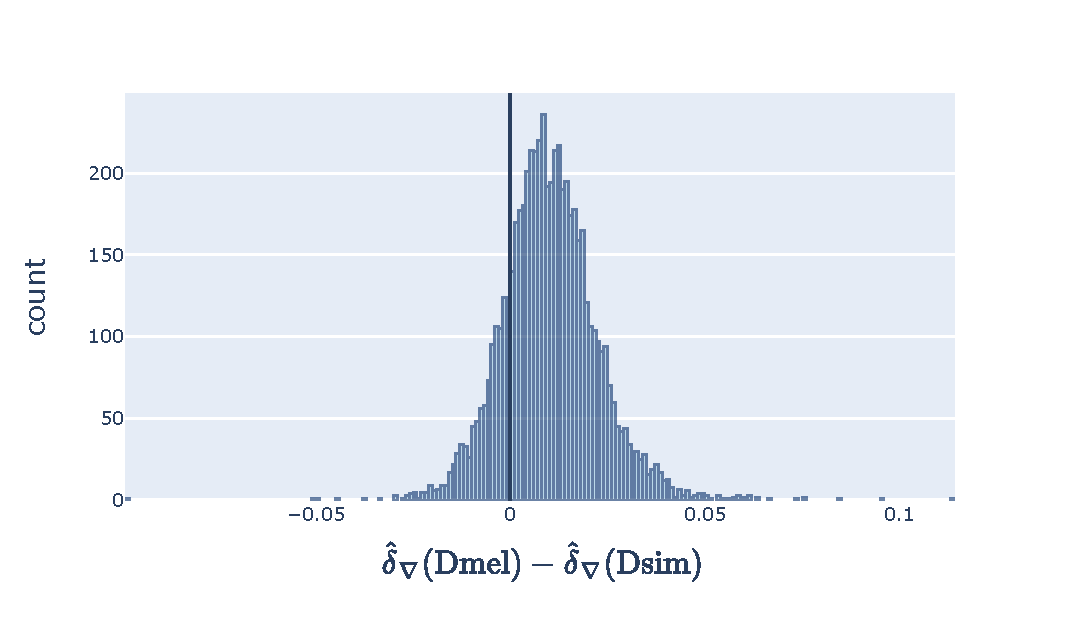
\includegraphics[width=	\textwidth]{figures/plots/drosophila/d-conv-diff.pdf}
\caption{\textbf{The magnitude of mutation disequilibrium is higher in \textit{D. melanogaster} genes.} }
\label{fig:drosophila_d-conv-diff}
\end{figure}


The pattern of elevated mutation disequilibrium is systematic across the \textit{D. melanogaster} genome. The median $\hat \delta_\nabla$ for a chromosome is shown with a horizontal line in Figure \ref{fig:drosophila_d-conv_manhattan}, where for all chromosomes analysed, \textit{D. melanogaster} clearly exceeds \textit{D. simulans}. Between the species, an unpaired $t$-test was performed on the same chromosome (e.g., Chromosome 2 in \textit{D. melanogaster} and Chromosome 2 in \textit{D. simulans}). The null hypothesis was that, for a given chromosome, the two species has the same mean $\hat\delta_\nabla$. The extremely low $p$-values for all comparisons ($\leq10^{-117}$) is very strong evidence against this null hypothesis (Table \ref{unpaired-t-dconv}). The consistency of elevation throughout the genome is in accordance with prior predictions

Strong purifying selection appears to impede the rate of convergence of the X chromosome. Considering that the X chromosome has fewer data points, it is evident in Figure \ref{fig:drosophila_d-conv-diff} that the \textit{D. melanogaster} X has a larger proportion of high $\hat \delta_\nabla$ than all other chromosomes shown. The median $\hat \delta_\nabla$ for Chromosomes 2, 3 and X in \textit{D. melanogaster} is $0.0132$, $0.0131$ and $0.0177$ respectively. The median $\hat \delta_\nabla$ for Chromosomes 2, 3 and X in \textit{D. simulans} is $0.0031$, $0.0031$ and $0.0040$ respectively. Within a species, an unpaired $t$-test was performed between chromosomes (e.g., Chromosome 2 and X in \textit{D. melanogaster}). All comparisons between an autosome and the X chromosome of the same species were significant, however, comparisons of the two autosomes of the same species were not (Table \ref{unpaired-t-dconv}). This is consistent with a slower rate of convergence and thus a higher magnitude of disequilibrium for sequence acted upon by purifying selection. 

\begin{figure}[htbp]
\centering
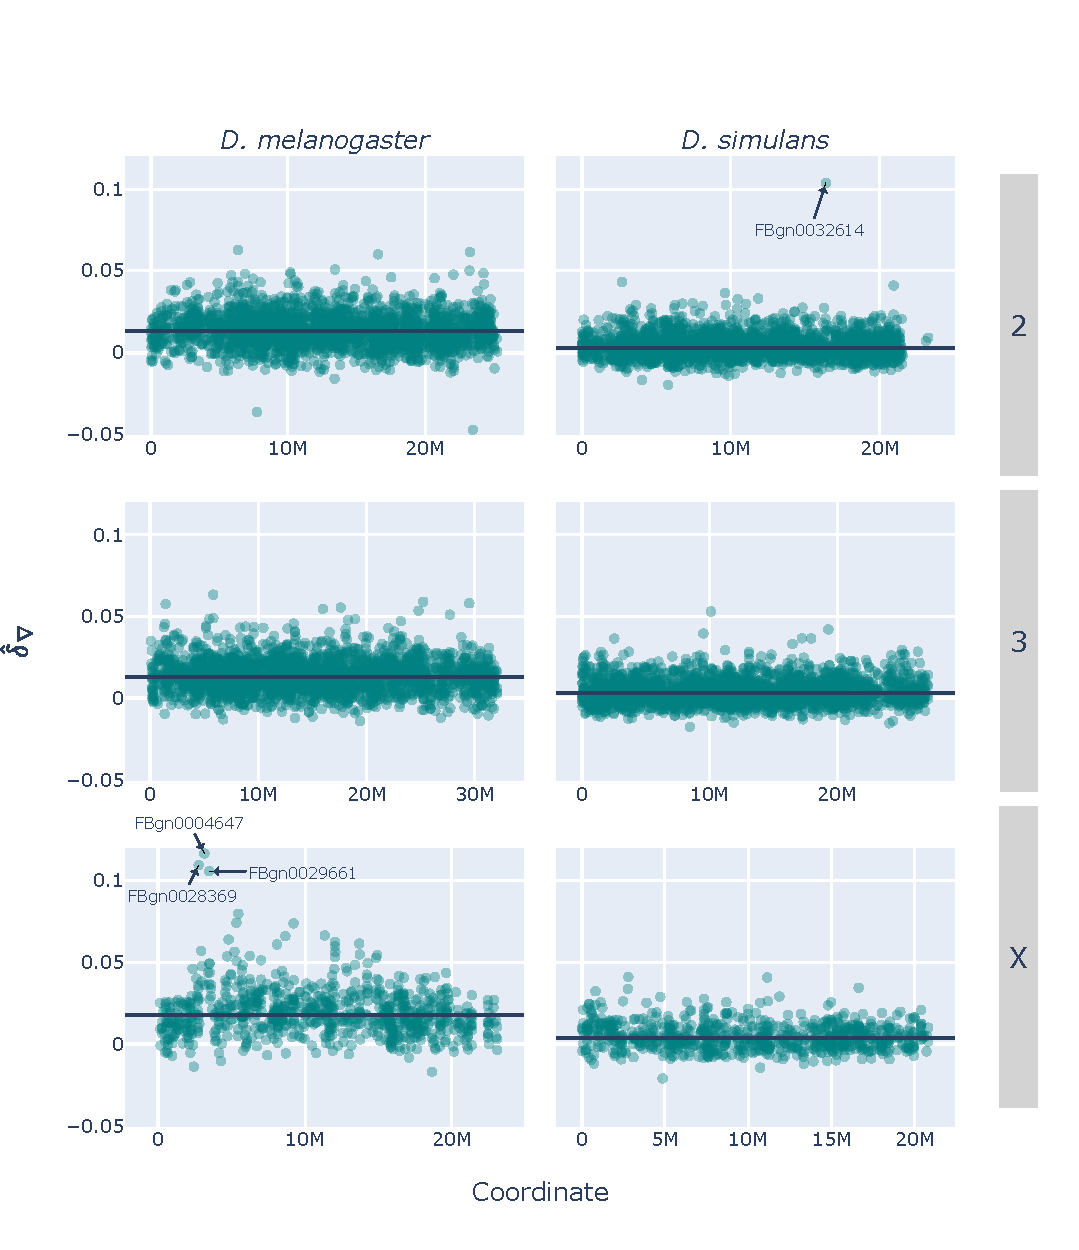
\includegraphics[width=\textwidth]{figures/plots/drosophila/d-conv_manhatten.pdf}
\caption{\textbf{The pattern of elevated mutation disequilibrium in \textit{D. melanogaster} compared to \textit{D. simulans} is systematic across the genome}. Manhattan plots the position of a gene in a chromosome and the $\hat\delta_\nabla$ for the CDS sequence of that gene. The CDS sequence is third codon position only. The median $\hat\delta_\nabla$ is indicated for a chromosome with a horizontal line. The number of genes included in the plots of chromosome 2, 3, and X of \textit{D. melanogaster} is 2373, 2624 and 818 respectively. For chromosome 2, 3, and X of \textit{D. simulans}, the number of genes is 2388, 2623 and 800 respectively.}
\label{fig:drosophila_d-conv_manhattan}
\end{figure}


\begin{table}[htbp]
\centering
\setstretch{1.3}
\begin{tabularx}{0.8\textwidth}{ 
  | >{\centering\arraybackslash}c
  | >{\centering\arraybackslash}X
  | >{\centering\arraybackslash}X | }
\hline  
Comparison & Test Statistic & $\hat p$-value \\
\hline 
    Dmel Chr X vs Dmel Chr 2 & -12.3 & 4.9e-34  \\
    Dmel Chr X vs Dmel Chr 3 & -12.7 & 1.8e-36  \\ 
    Dmel Chr 2 vs Dmel Chr 3 & -0.4 & 7.8e-1  \\ 
    Dsim Chr X vs Dsim Chr 2 & -2.6 &  9.9e-3  \\
    Dsim Chr X vs Dsim Chr 2 & -2.4 &  1.8e-2  \\
    Dsim Chr 2 vs Dsim Chr 3 & -0.2 & 8.1e-1  \\ 
    Dmel Chr 2 vs Dsim Chr 2 & 37.0 &  1.1e-263  \\
    Dmel Chr 3 vs Dsim Chr 3 & 40.2 &  1.0e-307  \\
    Dmel Chr X vs Dsim Chr X & 25.1 &  2.9-117  \\

\hline 
\end{tabularx}
\caption{\textbf{Unpaired $t$-test between \textit{Drosophila} chromosomes.} The 2-sample test is performed between pairs of Chromosome (Chr) 2, 3 and X of \textit{D. melanogaster} (Dmel) and \textit{D. simulans} (Dsim). }
\label{unpaired-t-dconv}
\doublespacing
\end{table}


The temporal EOP test did not reject equivalence between the majority of \textit{D. melanogaster} and \textit{D. simulans} genes. In the Q-Q plot comparing the distribution of tEOP $p$-values to the uniform distribution, (Figure \ref{fig:drosophila:temp-EOP-qq}), data points are close to the diagonal line, indicating a high level of similarity between the distributions. The estimate of the proportion of genes for which the process was not equivalent was 5\%.

\begin{figure}[ht!]
\centering
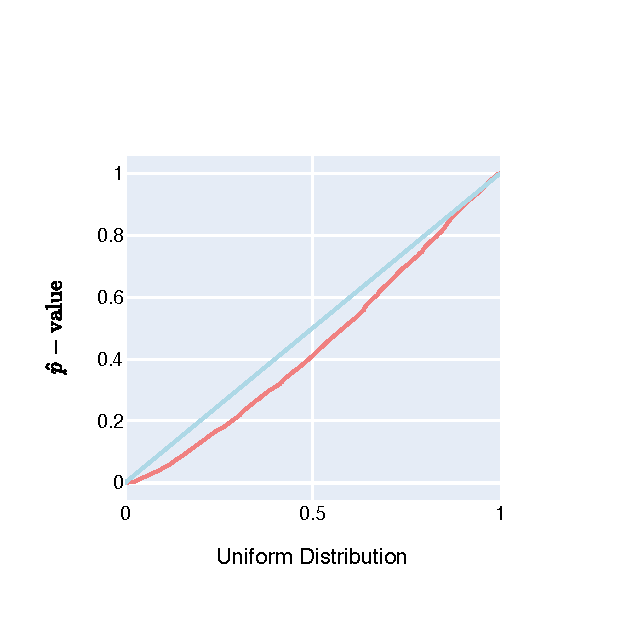
\includegraphics[width=0.6\textwidth]{figures/plots/drosophila/temp-EOP-QQ.pdf}
\caption[The mutagenic process was not distinguishable between \textit{D. melanogaster} and \textit{D. simulans}]{\textbf{The mutagenic process was not distinguishable between \textit{D. melanogaster} and \textit{D. simulans}.} The Quantile-Quantile plots compare the distribution of the temporal EOP between genes in \textit{D. melanogaster} and their ortholog in \textit{D. simulans} to  to the uniform distribution. The data points fall close to the diagonal indicating that the distribution is almost identical to what we would expect if the null was true. The plot shows 5,942 third codon position CDS alignments from \textit{D. melanogaster}, \textit{D. simulans} and \textit{D. yakubra}. }
\label{fig:drosophila:temp-EOP-qq}
\end{figure}


\section{Testing the conjectured}

Recombination and its association with GC-biased gene conversion has been proposed to be a major force in the formation of isochores \citep{Montoya-Burgos2003RecombinationGenomes}. The translocation of \textit{Fxy} in \textit{M. musculus} such that half of the gene now resides in the only part of the X chromosome that recombines with the Y is a natural experiment from which that conjecture may be tested. This perturbation was predicted to exhibit elevated disequilibrium in the PAR located section relative to the X-specific section (Figure \ref{fig:Fxy}). To test this prediction I used alignments of \textit{Fxy} in \textit{M. musculus} with orthologs from \textit{M. spretus} and \textit{R. norvegicus}. For all model fitting, \textit{M. musculus} was the foreground edge. I analysed the first six introns of \textit{Fxy}, of which in \textit{M. musculus} the $5'$ end (exons 1-3) is X-specific, and the $3'$ end (exons 4-6) is located in the PAR. The boundary of the PAR is found in the third intron \citep{Palmer1997AMice}. 

I aimed to determine whether the current understanding of how this translocation may affect the divergence process would be reflected by the methods. Because the entire gene had been translocated, I expected the whole gene to be in mutation disequilibrium. Considering the distinct mutagenic properties of the PAR, I aimed to see whether by using the statistic of magnitude, $\delta_\nabla$, I could detect elevated levels of disequilibrium in the PAR-located half. A specific location of the boundary is not provided. Therefore, I aimed to see whether the magnitude of mutation disequilibrium locally within intron 3 would illustrate where the boundary is located. 

\subsection{The PAR-half of \textit{Fxy} has elevated mutation disequilibrium relative to the X-linked half in \textit{M. musculus}}
\label{Fxy_TOE}

Although the entire \textit{Fxy} gene is in mutation disequilibrium (Table \ref{table:nablaFxy}), the magnitude of mutation disequilibrium was substantially higher in the PAR section relative to the X-specific. The aEOP test between neighbouring introns revealed introns 1-4 evolve by significantly different processes, however, adjacent comparisons between introns 4-6 did not reject the null. As most neighbouring introns rejected the null of equivalence in the aEOP test, I looked at each intron separately. All introns had a $\hat p$-value of $\leq 0.01$. The $\delta_\nabla$ statistic showed a clear difference between the two regions. Introns in the PAR (4-6) had $\hat\delta_\nabla$ markedly higher than those that are X-specific (1-2). The smallest $\hat \delta_\nabla$ in the PAR (intron 5) was 19 times larger than the largest $\hat \delta_\nabla$ that was X-specific (intron 2).

\begin{table}[htbp]

\begin{center}
\setstretch{1.6}
\begin{tabularx}{\textwidth}[t]{ 
  | >{\centering\arraybackslash}c 
  | >{\centering\arraybackslash}X 
  | >{\centering\arraybackslash}X  
  | >{\centering\arraybackslash}X  
  | >{\centering\arraybackslash}X  
  | >{\centering\arraybackslash}X  
  | >{\centering\arraybackslash}X | 
  }
\hline
\textbf{{Intron Rank}} & \textbf{{1}} & \textbf{{2}} & \textbf{{3}} & \textbf{{4}} & \textbf{{5}} & \textbf{{6}} \\
\hline
ToE $\hat p$-value & 0.00 & 0.00 & 0.01 & 0.00 & 0.00 & 0.00 \\
\hline
$\hat\delta_\nabla$ & 0.0019 & 0.0024 & 0.0115 & 0.0490 & 0.0470 & 0.0671 \\
\hline
\end{tabularx}
\end{center}
\caption{\textbf{The magnitude of mutation disequilibrium is highest in the region of the \textit{Fxy} gene that resides in the PAR.}}
\label{table:nablaFxy}

\end{table}

There is a clear difference in $\hat \delta_\nabla$ either side of intron 3. The portion of the gene $5'$ to intron 3 is X-specific, while the $3'$ portion is located in the PAR. This result motivated a closer analysis of intron 3 to try and identify a ``breakpoint'' at which the process shifts. To tackle this aim I performed a sliding window $5' \rightarrow 3'$ along the alignment of intron 3, computing $\hat \delta_\nabla$ for each window. The window took $600$ positions of the raw alignment, excluded alignment positions as described in the methods (Section \ref{Data Filtering}), and if at least 300 positions remained, computed $\hat \delta_\nabla$. 

Sliding window analysis showed that $\delta_\nabla$ oscillates within intron 3, with the amplitude of the oscillation largest at the $3'$ end (Figure \ref{fig:rodent/d-conv/intron3_4}a). For each window, $\hat \delta_\nabla$ is plotted against the location of the window midpoint, noting that the location is with respect to \textit{M. musculus}. The location of annotated repeats in \textit{M. musculus} are shown on the bottom of the figure, of which the different colours simply indicate different classes of repeats. The figure shows a period of oscillation in $\hat \delta_\nabla$ that is considerably consistent across the intron. These local fluctuations meant that the aim of determining a breakpoint could not be so simply met. Remarkably, the local fluctuations still exhibit a marked increase in amplitude towards the $3'$ end of the intron. This is of considerable interest, although the underlying process has repetitive local changes, there is still an identifiable change in the process in the region of the intron expected to be in the PAR. 

The oscillation appeared to be more consistent in intron 4, which is located in the PAR (Figure \ref{fig:rodent/d-conv/intron3_4}b). Using signal processing techniques I estimated the dominant oscillation length to be $\sim1470$. The oscillation is a feature of \textit{Fxy} introns, although to differing extents (data shown in appendices.) (ref) 

\begin{figure}[htbp]
\centering
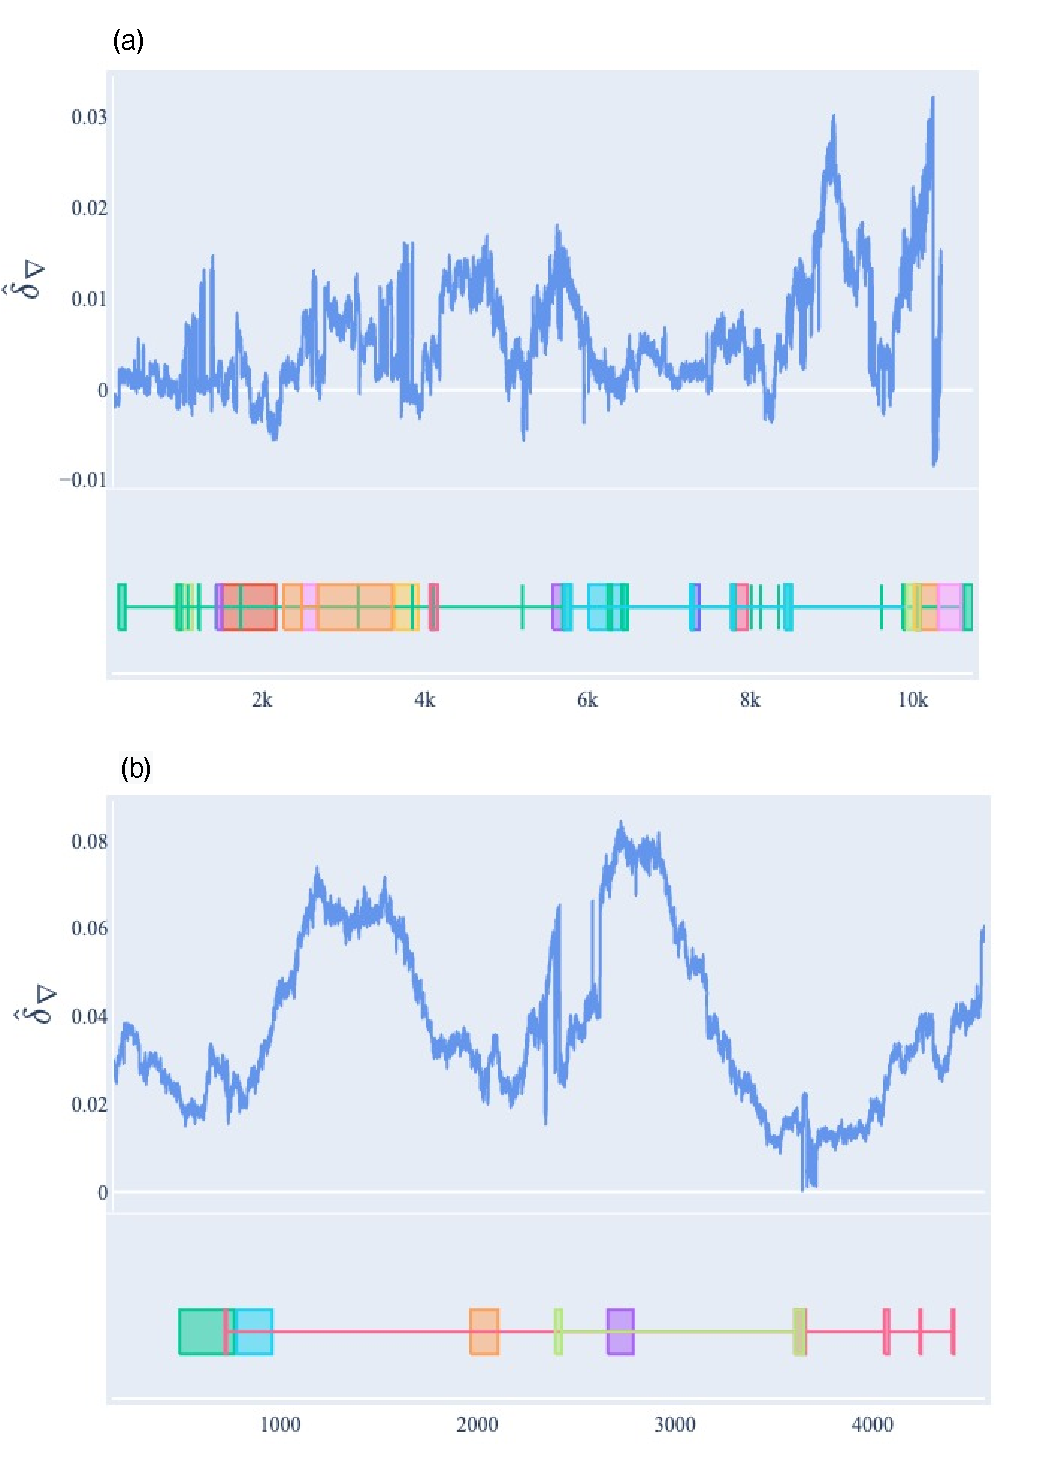
\includegraphics[width=\textwidth]{figures/plots/rodent/dconv-intron3_4.pdf}
\caption{\textbf{Moving average of $\hat\delta_\nabla$ in intron 3 of \textit{Fxy}.} The scatter plot shows the position of the mid point of a `sliding window' across the intron against the smoothed moving average of $\hat\delta_\nabla$. The location of annotated repeats in the \textit{M. musculus} sequence are indicated with the segments at the bottom of the figure. Different colours simply indicate different classes of repeats. The window looked at 600 positions of the raw alignment, and calculated $\hat\delta_\nabla$ if more than 300 positions remained after filtering. The taxa included in the alignment were \textit{M. musculus}, \textit{M. spretus}, and \textit{R. norvegicus}. In all model fitting \textit{M. musculus} was considered the foreground edge. }
\label{fig:rodent/d-conv/intron3_4}
\end{figure}

The conjectured impact of recombination on the divergence of sequence located within the PAR is reflected in these developed methods. The results show that although the entire translocated \textit{Fxy} gene rejected the null of mutation equilibrium, the magnitude of disequilibrium was strongest in the section that is now located in the PAR. Within the introns there is a fascinating pattern of the magnitude of disequilibrium, furthermore, the entire pattern is magnified towards the PAR. These results support local rearrangements being a mechanism of mutation disequilibrium and that the more distinct the mutagenic environment in the new location, the higher the magnitude of mutation disequilibrium.

\section{Testing the unknown}

The effectiveness of the methods in the previous applications provides the grounds for the application to this unknown case. To test for the existence and measure the magnitude of mutation disequilibrium in the human genome, I used intronic and CDS alignments of human chromosome 1 linked genes and their orthologs in chimpanzee and gorilla. The CDS data was alignments of third codon positions only. 

\subsection{The majority of the human genome is in mutation disequilibrium}
\label{Human:TOE}
For both the intronic and CDS data, Q-Q plots indicated that there are a proportion of genes that are not in equilibrium (Figure \ref{fig:primate_lrt_qq}). I estimated the proportion of the sample consistent with the alternate hypothesis as $\sim50\%$ for intronic sequence, and $\sim68\%$ for CDS. It is important to note that an assumption of this method of estimation is that the data consistent with the null hypothesis is uniformly distributed. This was not the case for the CDS negative control (Figure \ref{fig:primate_lrt_qq}b). How this departure from the assumed distribution impacts the estimation of $f$ is unknown. 

\begin{figure}[h]
\centering
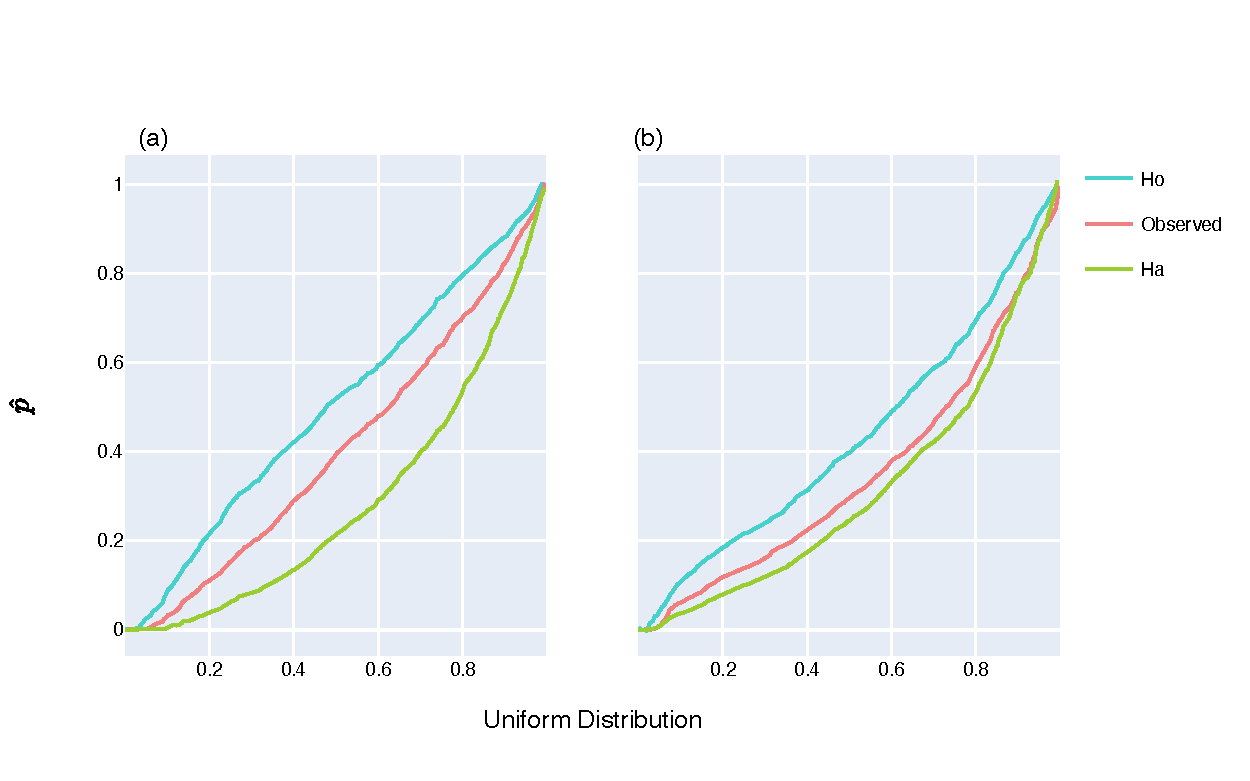
\includegraphics[width=	\textwidth]{figures/plots/primate/LRT-QQ.pdf}
\caption[Humans exhibit a higher proportion of mutation disequilibrium in CDS compared to introns]{\textbf{Humans exhibit a higher proportion of mutation disequilibrium in CDS compared to introns.} The Quantile-Quantile plots compare the distribution of $\hat p-$values to the expected uniform distribution. \textbf{(a)} 1,406 alignments of introns from human, chimpanzee and gorilla, \textbf{(b)}, 1,182 CDS alignments from human, chimpanzee and gorilla. For all model fitting human was the foreground edge. }
\label{fig:primate_lrt_qq}
\end{figure}


\subsection{Purifying natural selection impedes the rate of convergence}

The introns of a gene evolve faster than its exons. For most genes (56\%) the difference in ENS between introns and CDS on the human edge is negative, indicating a faster rate of evolution in intronic sequences (Figure \ref{fig:primate:dconv-diff}a). The distribution of the difference in $\hat\delta_\nabla$ is inversely distributed, 62\% is positive, indicating a greater magnitude of disequilibrium in CDS (Figure \ref{fig:primate:dconv-diff}b). It appeared that owing to a lesser selective constraint, intronic sequences seemed to be already closer to equilibrium. There are, however, a lot of genes for which this is not the case.

\begin{figure}[h]
\centering
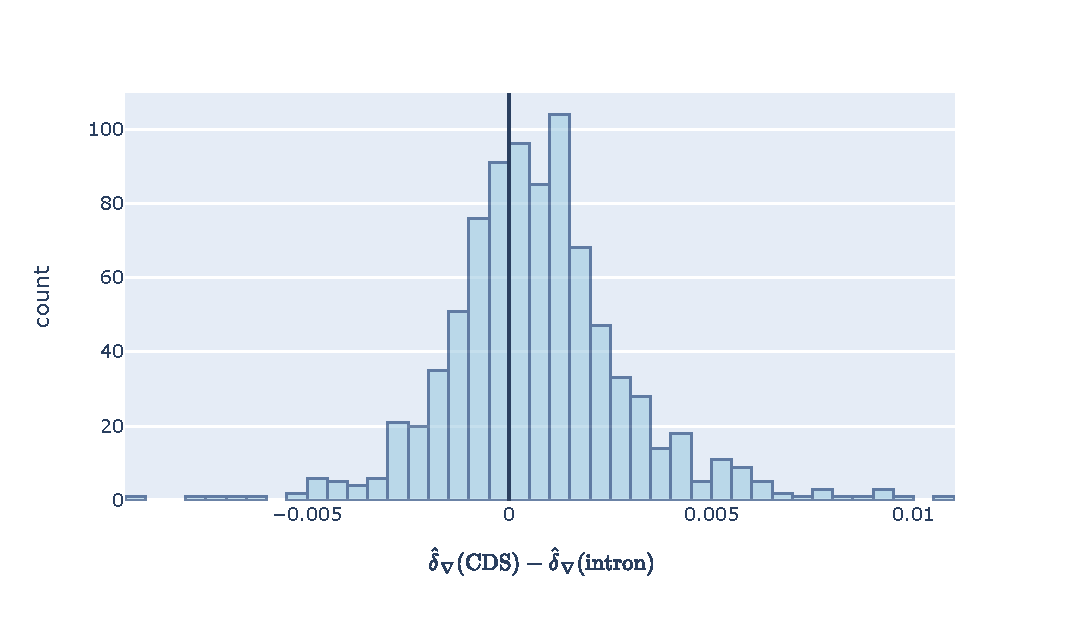
\includegraphics[width=	\textwidth]{figures/plots/primate/d-conv-diff.pdf}
\caption{}
\label{fig:primate:dconv-diff}
\end{figure}


The magnitude of disequilibrium is heterogeneous along a chromosome. Figure \ref{fig:primate:dconv-manhattan} shows $\hat \delta_\nabla$ plotted against the coordinate of the gene on the chromosome for both intronic and CDS. There are clear regions where the average magnitude of disequilibrium is higher than others, this is illustrated best by looking at the first 50M section of introns vs the next 50M section. Interestingly, the overall trend of $\hat \delta_\nabla$ is mirrored between the sequence types. 

\begin{figure}[htbp]
\centering
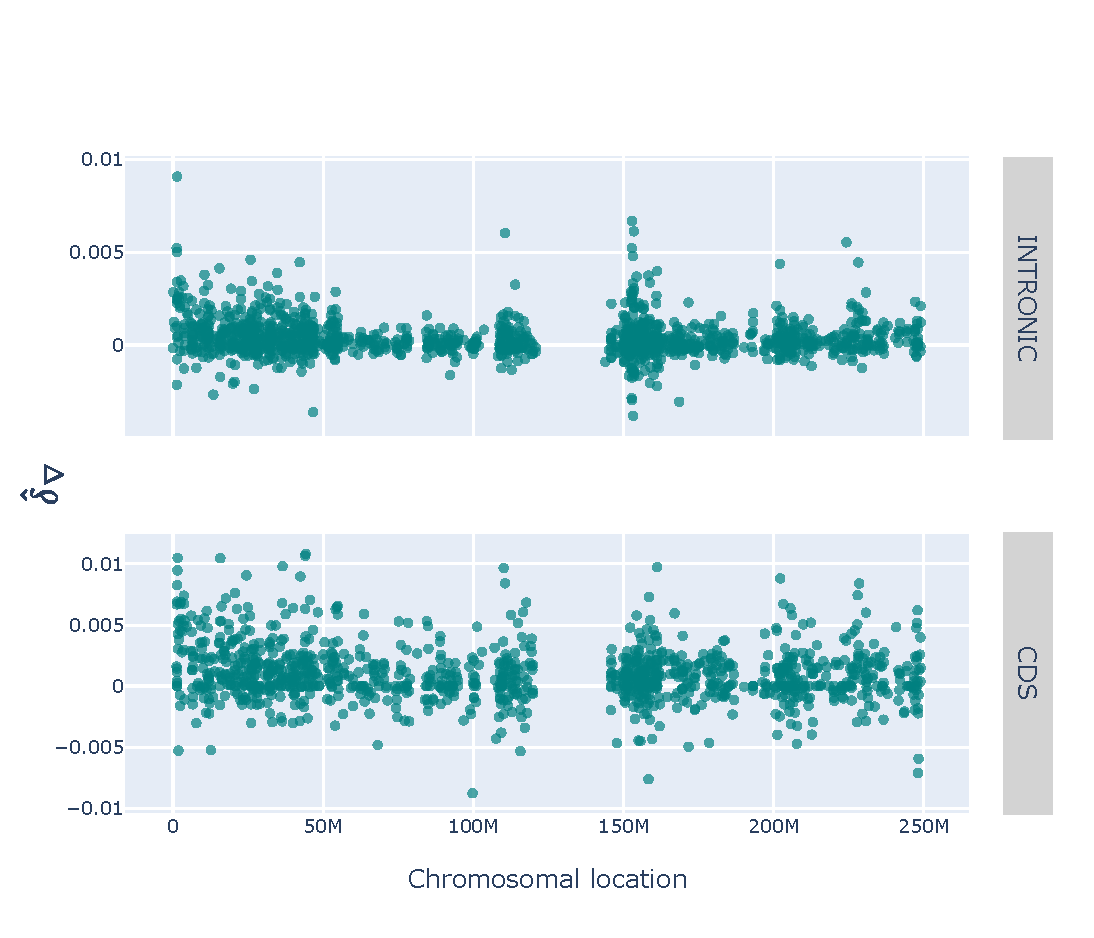
\includegraphics[width=	\textwidth]{figures/plots/primate/d-conv-manhatten.pdf}
\caption{\textbf{The magnitude of disequilibrium is heterogeneous along a chromosome.} Manhattan plots show the position of a gene in a chromosome and the $\hat\delta_\nabla$ for the intronic (top) and CDS sequence (bottom) of that gene. Intronic data included 1,406 alignments CDS data included 1,182. The taxa in all alignments were human, chimpanzee and gorilla, in all model fitting human was the foreground edge. }
\label{fig:primate:dconv-manhattan}
\end{figure}


The results from my analyses show that mutation disequilibrium is a pervasive feature of genomes and that the developed methods are effective in robustly detecting and measuring it. In \textit{D. melanogaster}, when DNA methylation with a well-established mutagenic effect was removed, you see a genome-wide increase in disequilibrium. In \textit{M. musculus}, the methods reflect elevated disequilibrium in the region that moved into the PAR, relative to the component of the gene that remains in the X-specific region. Applying the methods to Human evolution, I conservatively estimate that greater than 50\% of our genome is in mutation disequilibrium